\begin{frame}{Ensembling}
\begin{itemize}
    \item No single model is perfect. Different models make different types of errors.
    \item Let's visualize the predictions of two different models:
\end{itemize}
\begin{figure}
    \centering
    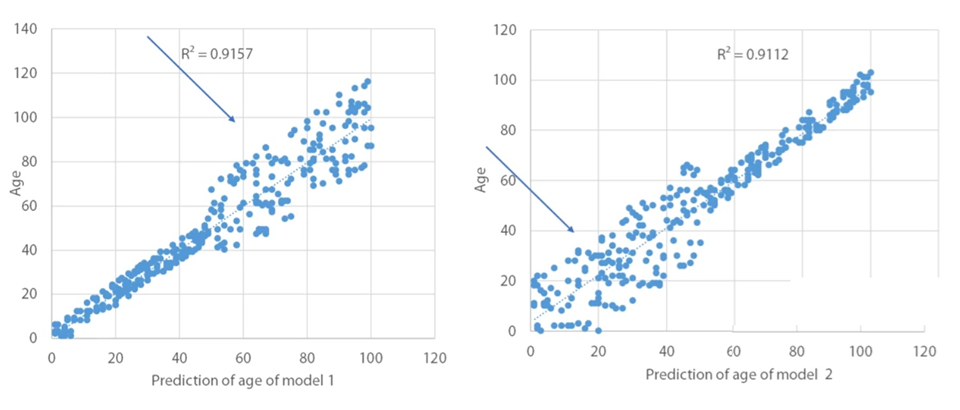
\includegraphics[width=1.0\linewidth,height=0.58\textheight,keepaspectratio]{images/ensembling1.png}
    \caption{Predictions of Model 1 and Model 2}
\end{figure}
\footnotetext{Figure: Coursera / HSE, ``How to Win a Data Science Competition: Learn from Top Kagglers'', week~4 ensembling lecture.}
\end{frame}

\begin{frame}{Ensembling}
\begin{itemize}
    \item Combining predictions of diverse models can reduce errors and improve accuracy. This technique is called \textbf{Ensembling}.
\end{itemize}
\begin{figure}
    \centering
    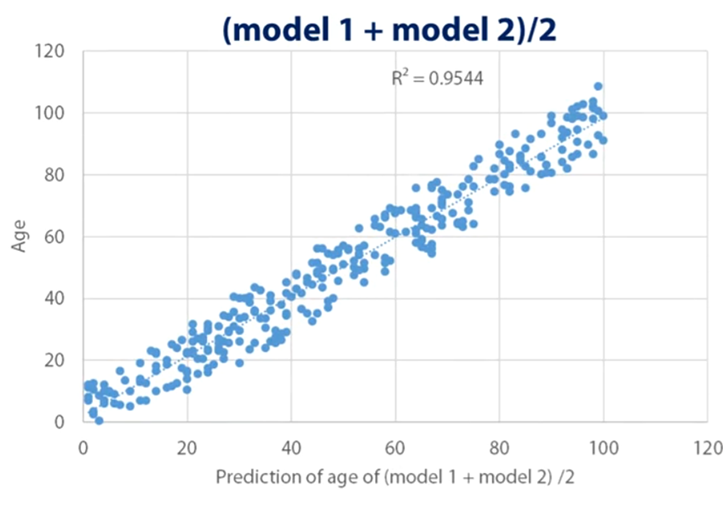
\includegraphics[width=0.7\linewidth,height=0.6\textheight,keepaspectratio]{images/ensembling2.png}
    \caption{Averaged Predictions: Better Correlation}
\end{figure}
\footnotetext{Figure: Coursera / HSE, ``How to Win a Data Science Competition: Learn from Top Kagglers'', week~4 ensembling lecture.}
\end{frame}

\begin{frame}{Ensembling}
\begin{itemize}
    \item Diverse models are key to effective ensembling. Here are two strategies:
    \begin{itemize}
        \item \textbf{Bagging (Bootstrap Aggregating):} Train multiple models on different subsets of data (e.g., Random Forest model).
    \end{itemize}
    \end{itemize}
    \begin{figure}
    \centering
    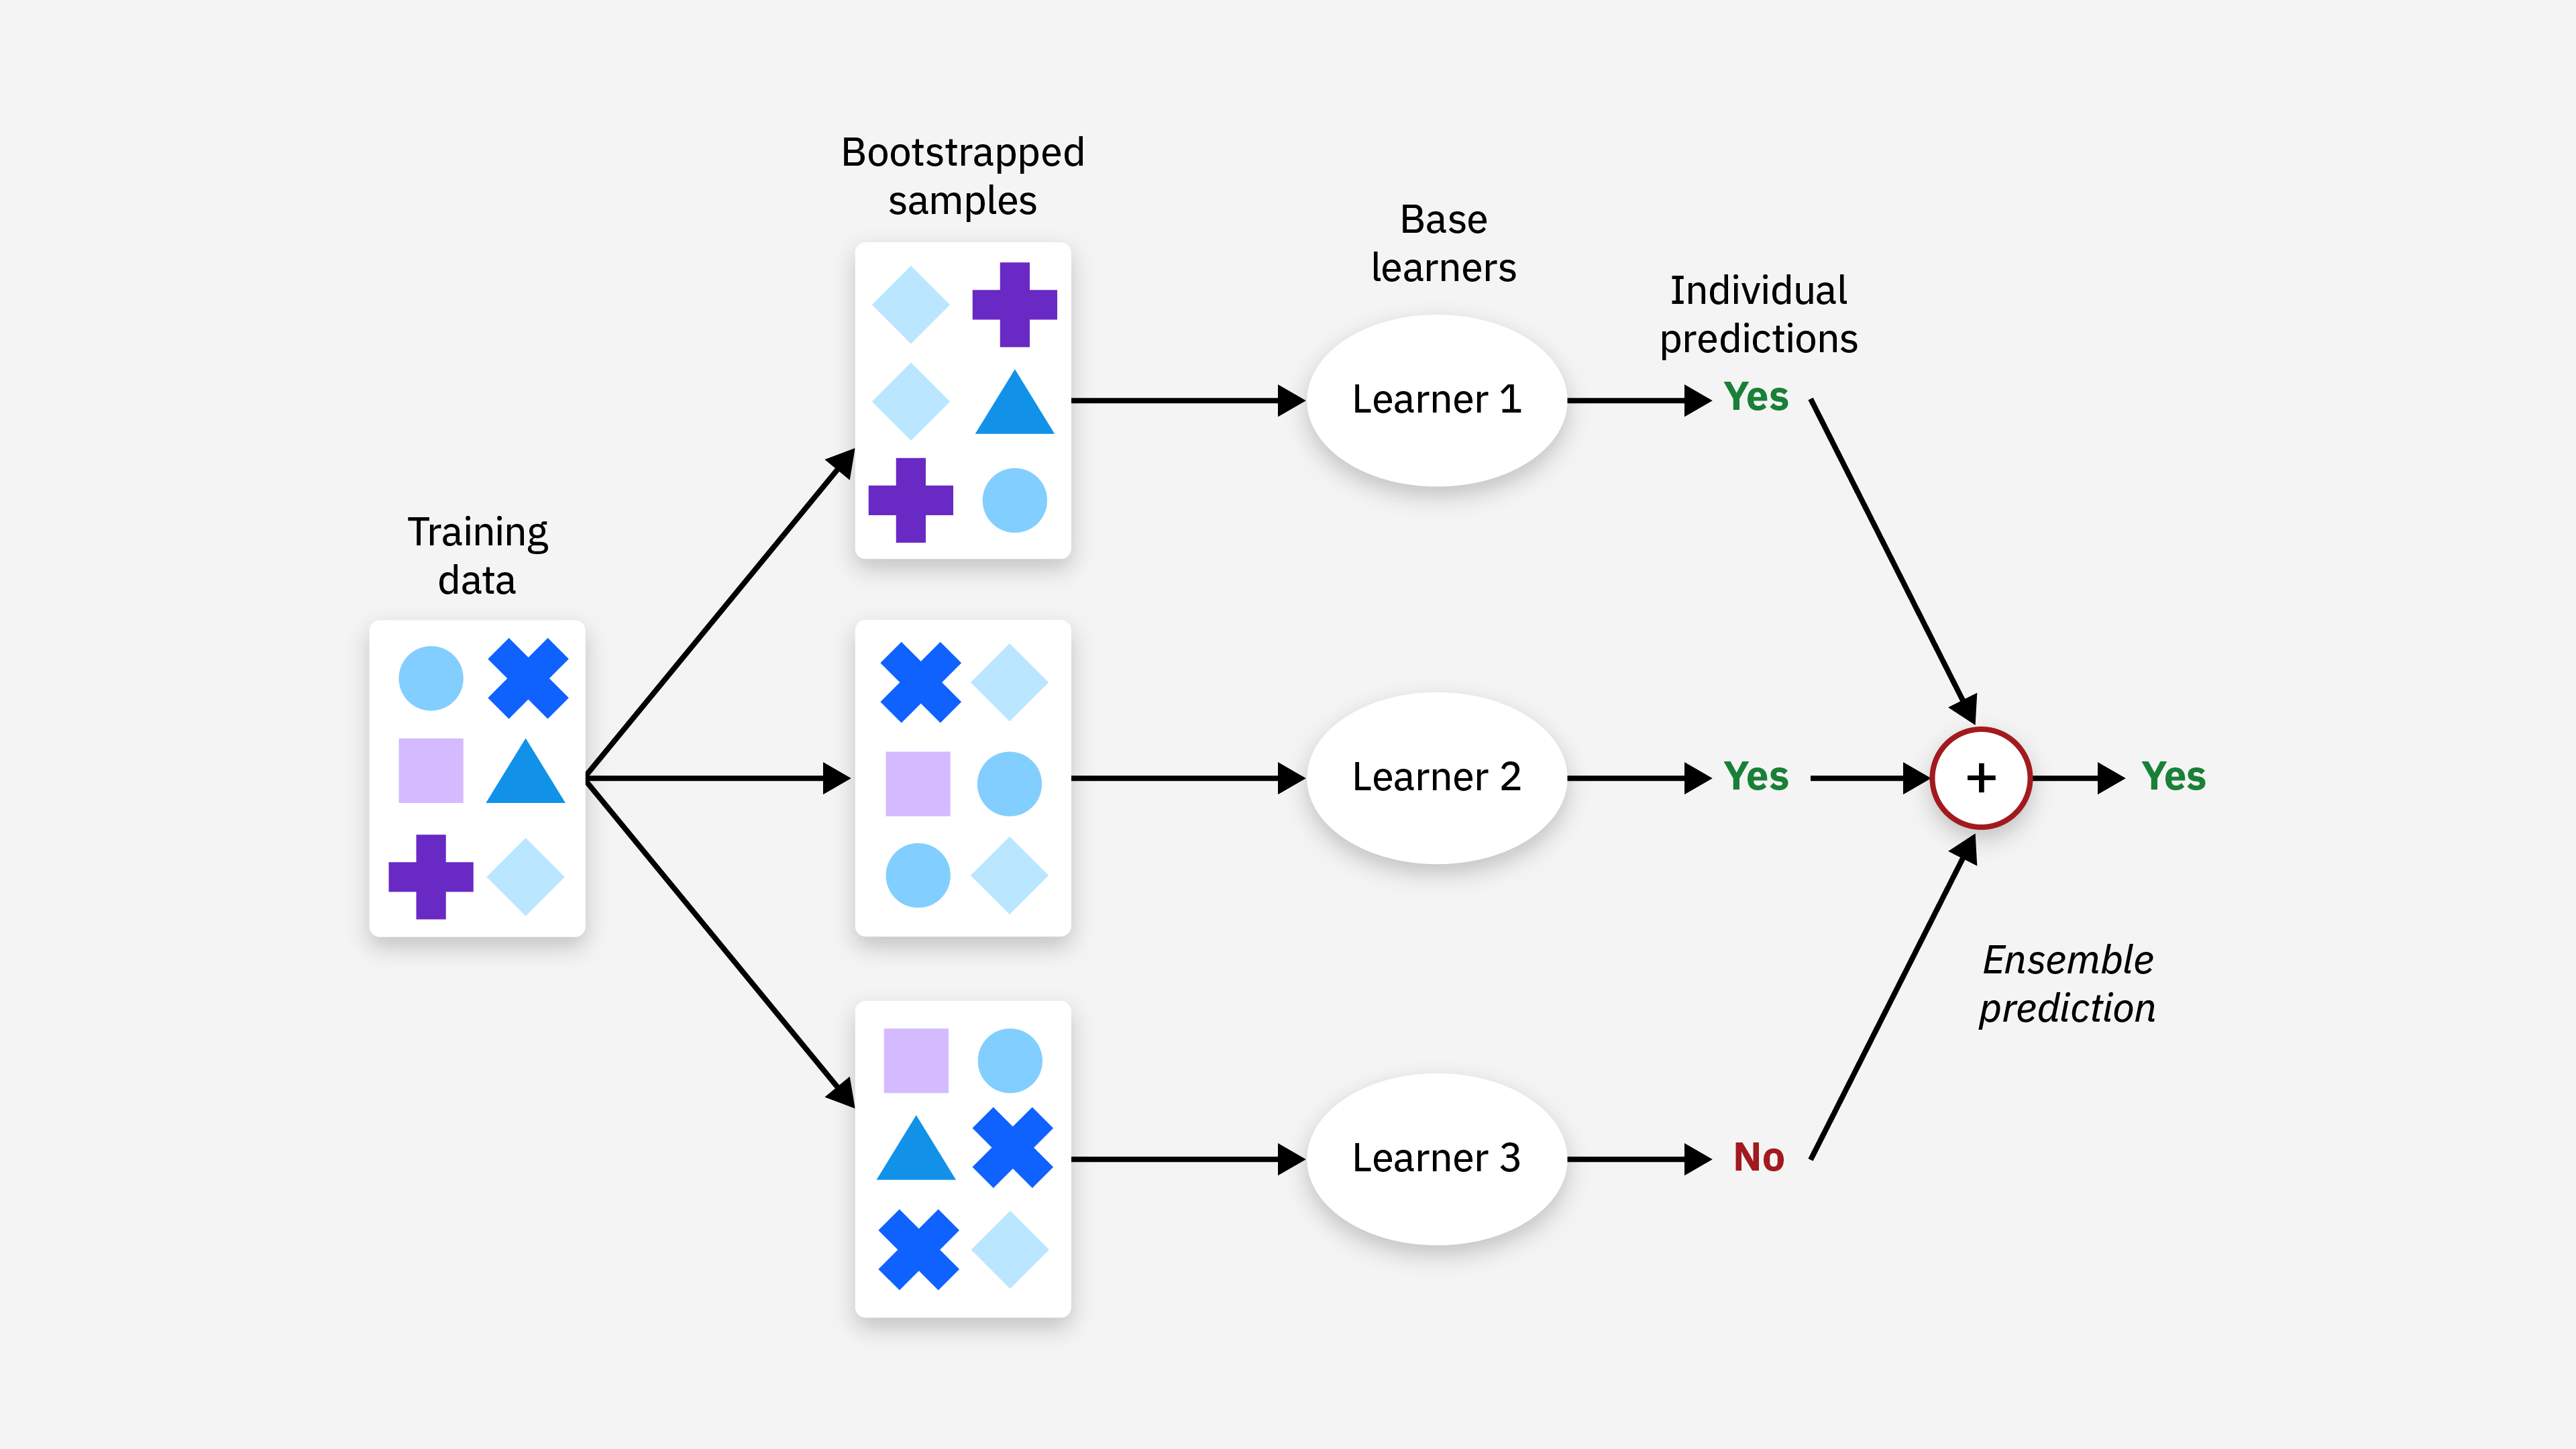
\includegraphics[width=0.8\textwidth,height=0.55\textheight,keepaspectratio]{images/bagging.png}
    \caption{Bagging example}
\end{figure}
\footnotetext{Figure: IBM, \url{https://www.ibm.com/think/topics/bagging}}
\end{frame}

\begin{frame}{Ensembling}
\begin{itemize}
    \item Boosting:
    \begin{itemize}
        \item Train models sequentially, where each model focuses on the errors of the previous one (e.g., AdaBoost, Gradient Boosting).
    \end{itemize}
\end{itemize}
\begin{figure}
    \centering
    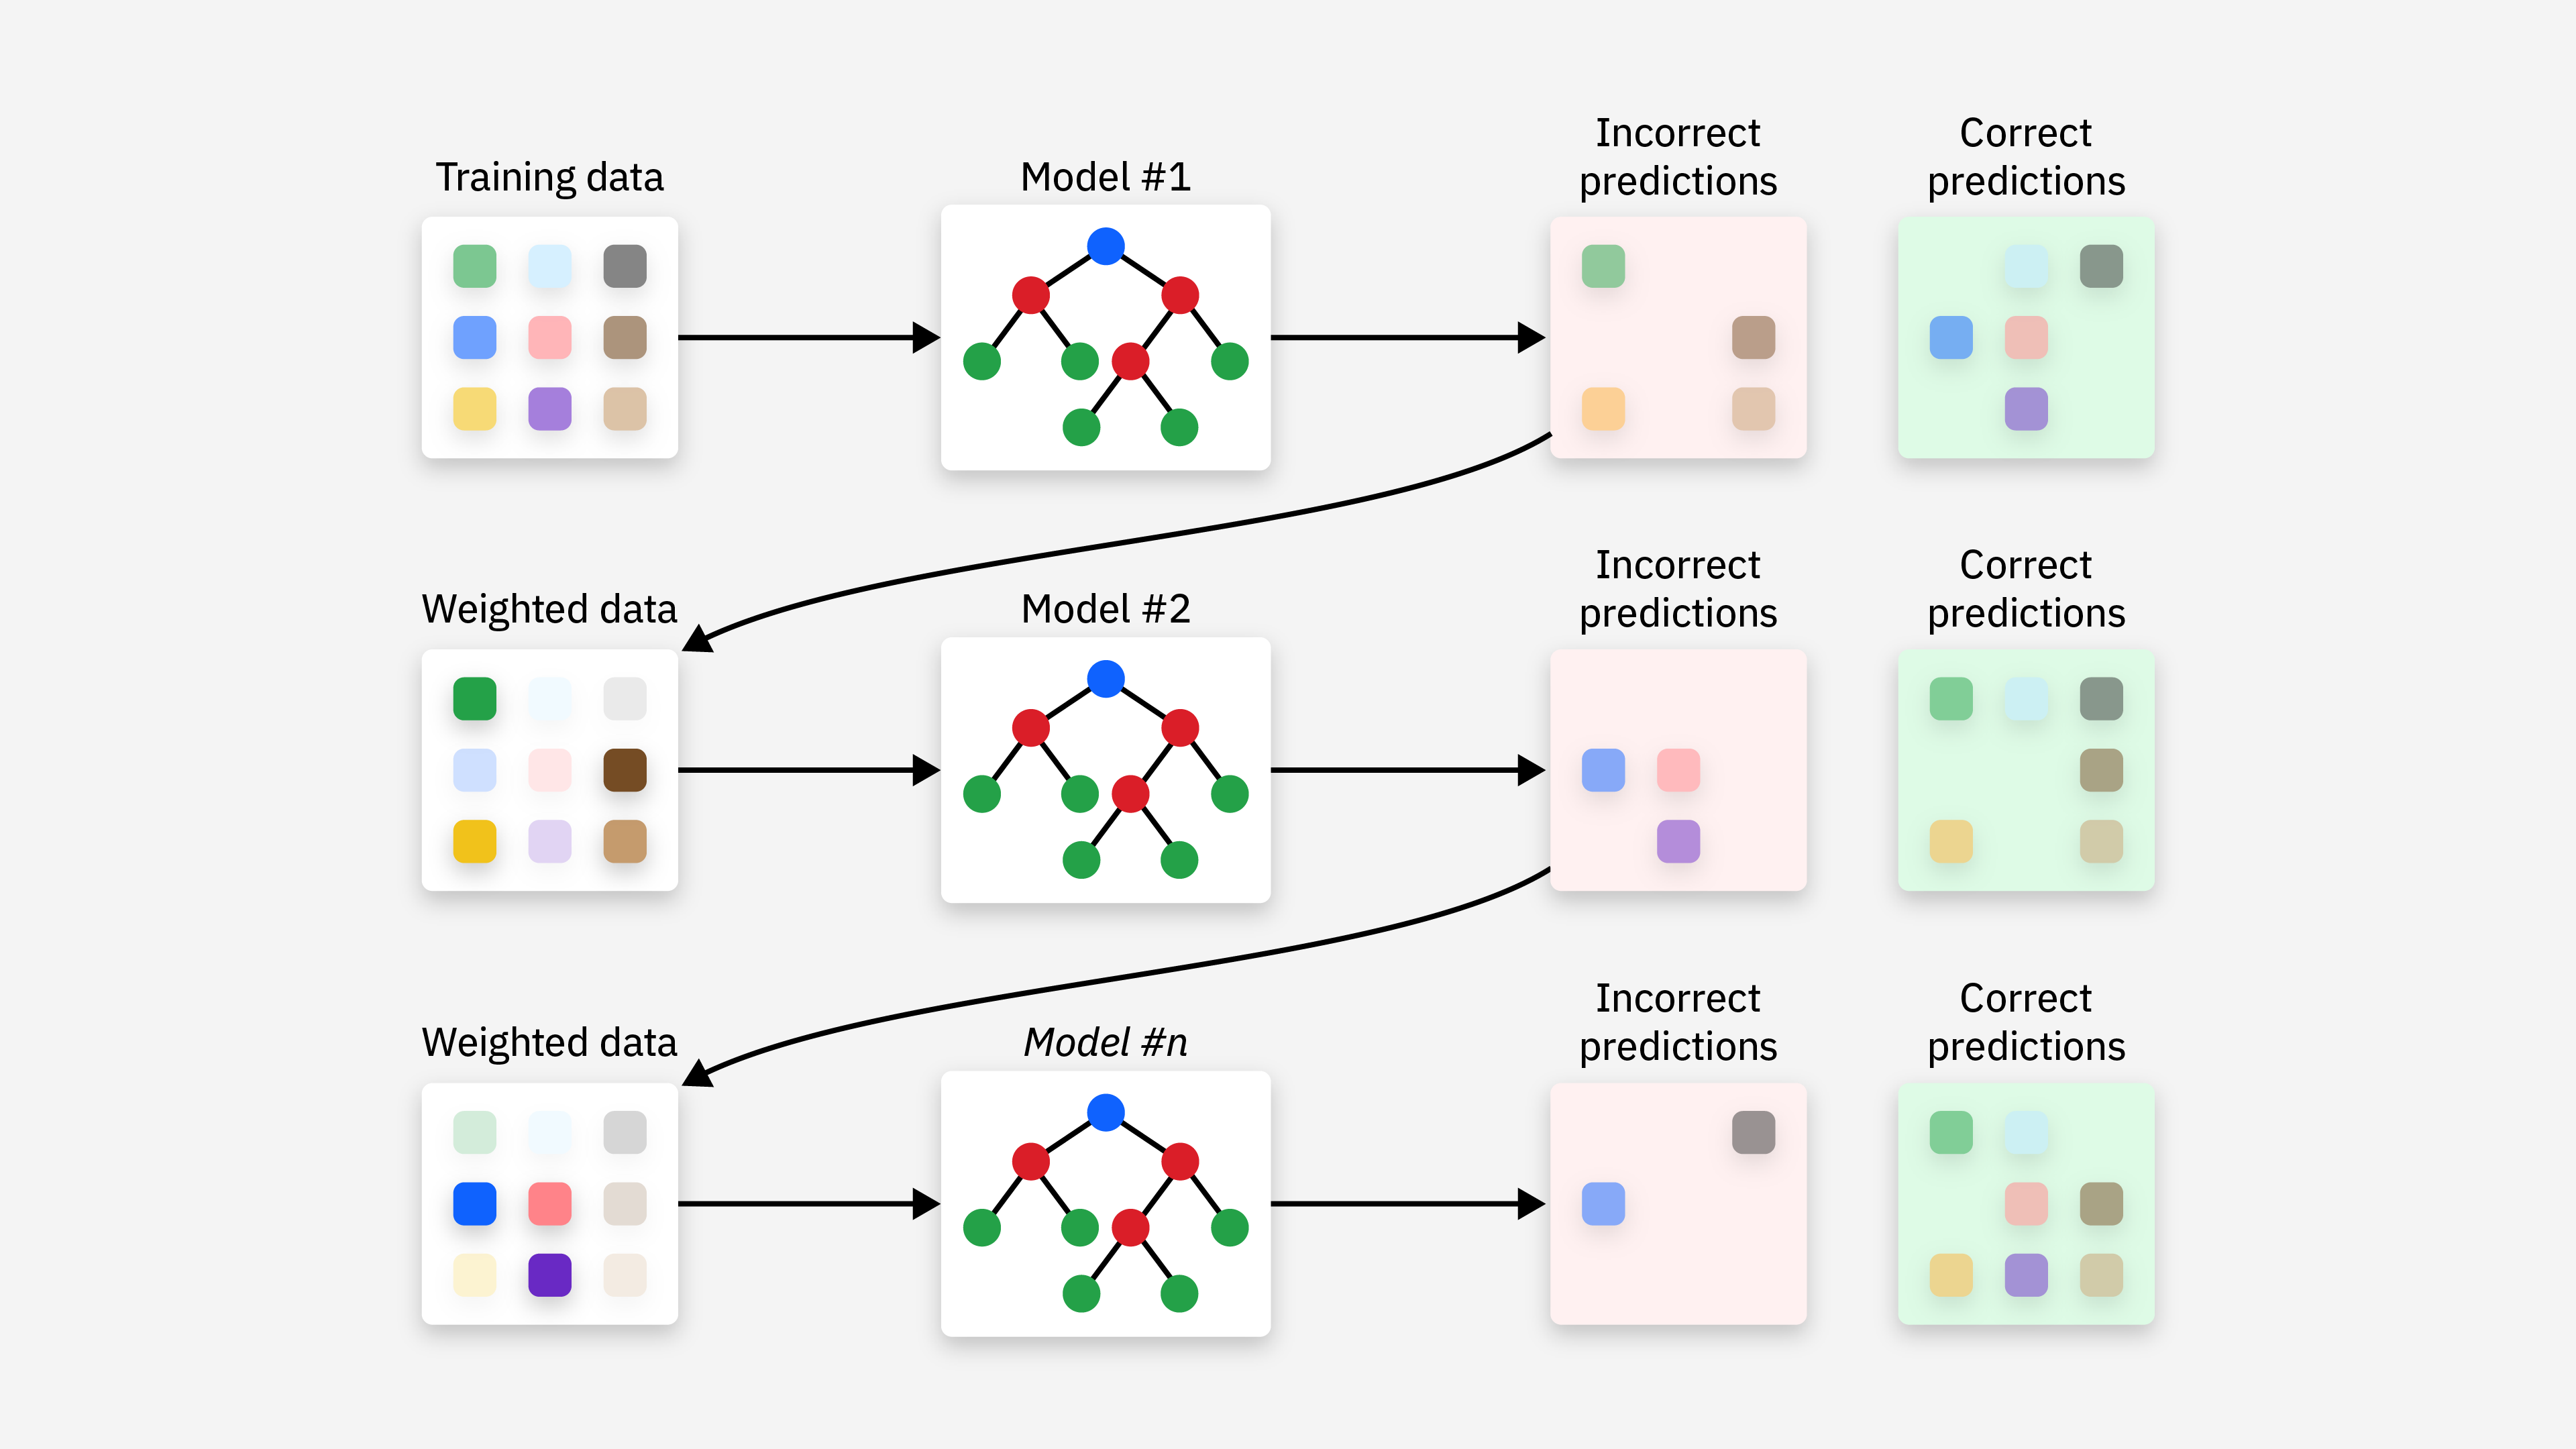
\includegraphics[width=0.8\textwidth,height=0.55\textheight,keepaspectratio]{images/boosting.png}
    \caption{Boosting Example}
\end{figure}
\footnotetext{Figure: IBM, \url{https://www.ibm.com/think/topics/boosting}}
\end{frame}

\begin{frame}{Ensembling}
\begin{itemize}
\item These strategies introduce diversity in models, but how can we combine their predictions?
\end{itemize}
\end{frame}

\begin{frame}{Ensembling}
\begin{itemize}
\item We can combine classifiers' predictions in two ways:
\begin{itemize}
    \item \textbf{Hard Voting:}
    \begin{itemize}
        \item Each model votes for a class.
        \item The class with the majority of votes is selected.
    \end{itemize}
    \item \textbf{Soft Voting:}
    \begin{itemize}
        \item Average the predicted probabilities from each model.
        \item The class with the highest average probability is selected.
    \end{itemize}
\end{itemize}
\item For regressors: take the average of predictions from all models.
\end{itemize}
\begin{figure}
    \centering
    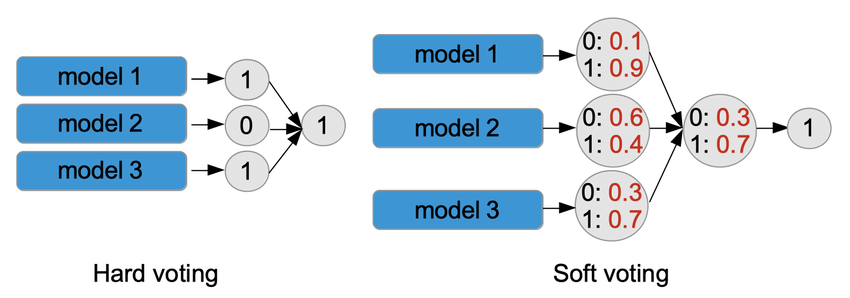
\includegraphics[width=0.4\linewidth,height=0.20\textheight,keepaspectratio]{images/voting.png}
    \caption{Illustration of Hard and Soft Voting for Classifiers}
\end{figure}
% NOTE: \' is bound to hyperref's PU encoding in this preamble and errors out in
% body text, so the acute i below uses TeX's \accent primitive instead.
\footnotetext{Figure: Bulaty Tauil et al., \href{https://doi.org/10.55905/oelv22n5-199}{Rev. Observatorio de la Econom\accent19 ia Latinoamericana} 22(5), 2024, Fig.~2.}
\end{frame}

\begin{frame}{Ensembling}
    \begin{itemize}
        \item Teamwork is the best policy.
        \item We can train multiple networks for the same task then ensemble to get better results.
    \end{itemize}
\end{frame}

\begin{frame}{Ensembling - A simple Analysis}
    \begin{itemize}
        \item Let's assume that we have a test dataset with $N$ elements and an ensemble of $M$ models.
        \item Also assume that each model in the ensemble errs independently on an image with the same probability, denoted by $e$.
        \item For example, assume $M=3$ and $e = 0.01$.
        \item Then the probability of error of the label for the max-voting ensemble will be
        $$p_{\text{ens}} = 1 - (1-e)^3 - \binom 32 (1-e)^2 e$$
        \item For the above example $p_{\text{ens}}=0.0003$, which is significantly lower than a single model.
    \end{itemize}
\end{frame} 